\section{Introduction}

Multimodal large language models (MLLMs)~\cite{qwen2vl,qwenvl,dong2025seedvl,internvl2,internvl2.5,luo2026next} are rapidly evolving from static input processors into interactive agents that can operate in digital and physical environments. In particular, vision-language-action (VLA) models~\cite{wang2024gui,nguyen2025gui,luo2025gui,gamescaling} offer a promising path toward embodied artificial general intelligence. However, high trial-and-error costs and the lack of environmental controllability significantly hinder both the evaluation and algorithm scaling of real-world physical agents.

Modern large-scale games~\cite{fan2022minedojo,baker2022vpt, gameverse, wang2026gamehorizon,towards,videoarena, gameworld2026,luo2026ai} provide an ideal testbed for developing generalist VLA agents and studying their scaling behaviors because they combine realistic complexity with rigorous experimental control. Compared with traditional 2D games, web interfaces, and simplified simulators, contemporary games require agents to parse complex visual scenes, navigate intricate 3D layouts, and advance multi-stage quests. Agents must continually make strategic decisions and manage resources under partial observability and delayed feedback, all through fine-grained, low-level keyboard and mouse actions. Tasks may last hours or longer, requiring reliable memory, planning, and decision-making throughout. Such environments therefore serve as an uncompromising benchmark for coordinating perception, reasoning, memory, and control.

\textit{Honkai: Star Rail} (HSR) exemplifies this setting by condensing these demands into a continuously evolving game environment. Its gameplay combines narrative-driven exploration across diverse regions with turn-based combat, squad management, resource allocation, and multi-level UI operation. This environment features nested objectives and long-term progression that challenge an agent's cross-task generalization, long-term memory, and closed-loop execution. Developing agents in this system compels MLLMs to transition from passive visual understanding to sustained, proactive interaction. Mastering such challenges paves a concrete pathway toward generalist agents capable of operating across both complex digital worlds and embodied physical environments. As illustrated in Figure~\ref{fig:overview}, \ourmodel is designed to operate across visually and mechanically diverse environments via a single screen-to-action interface.

\begin{figure*}[!t]
\centering
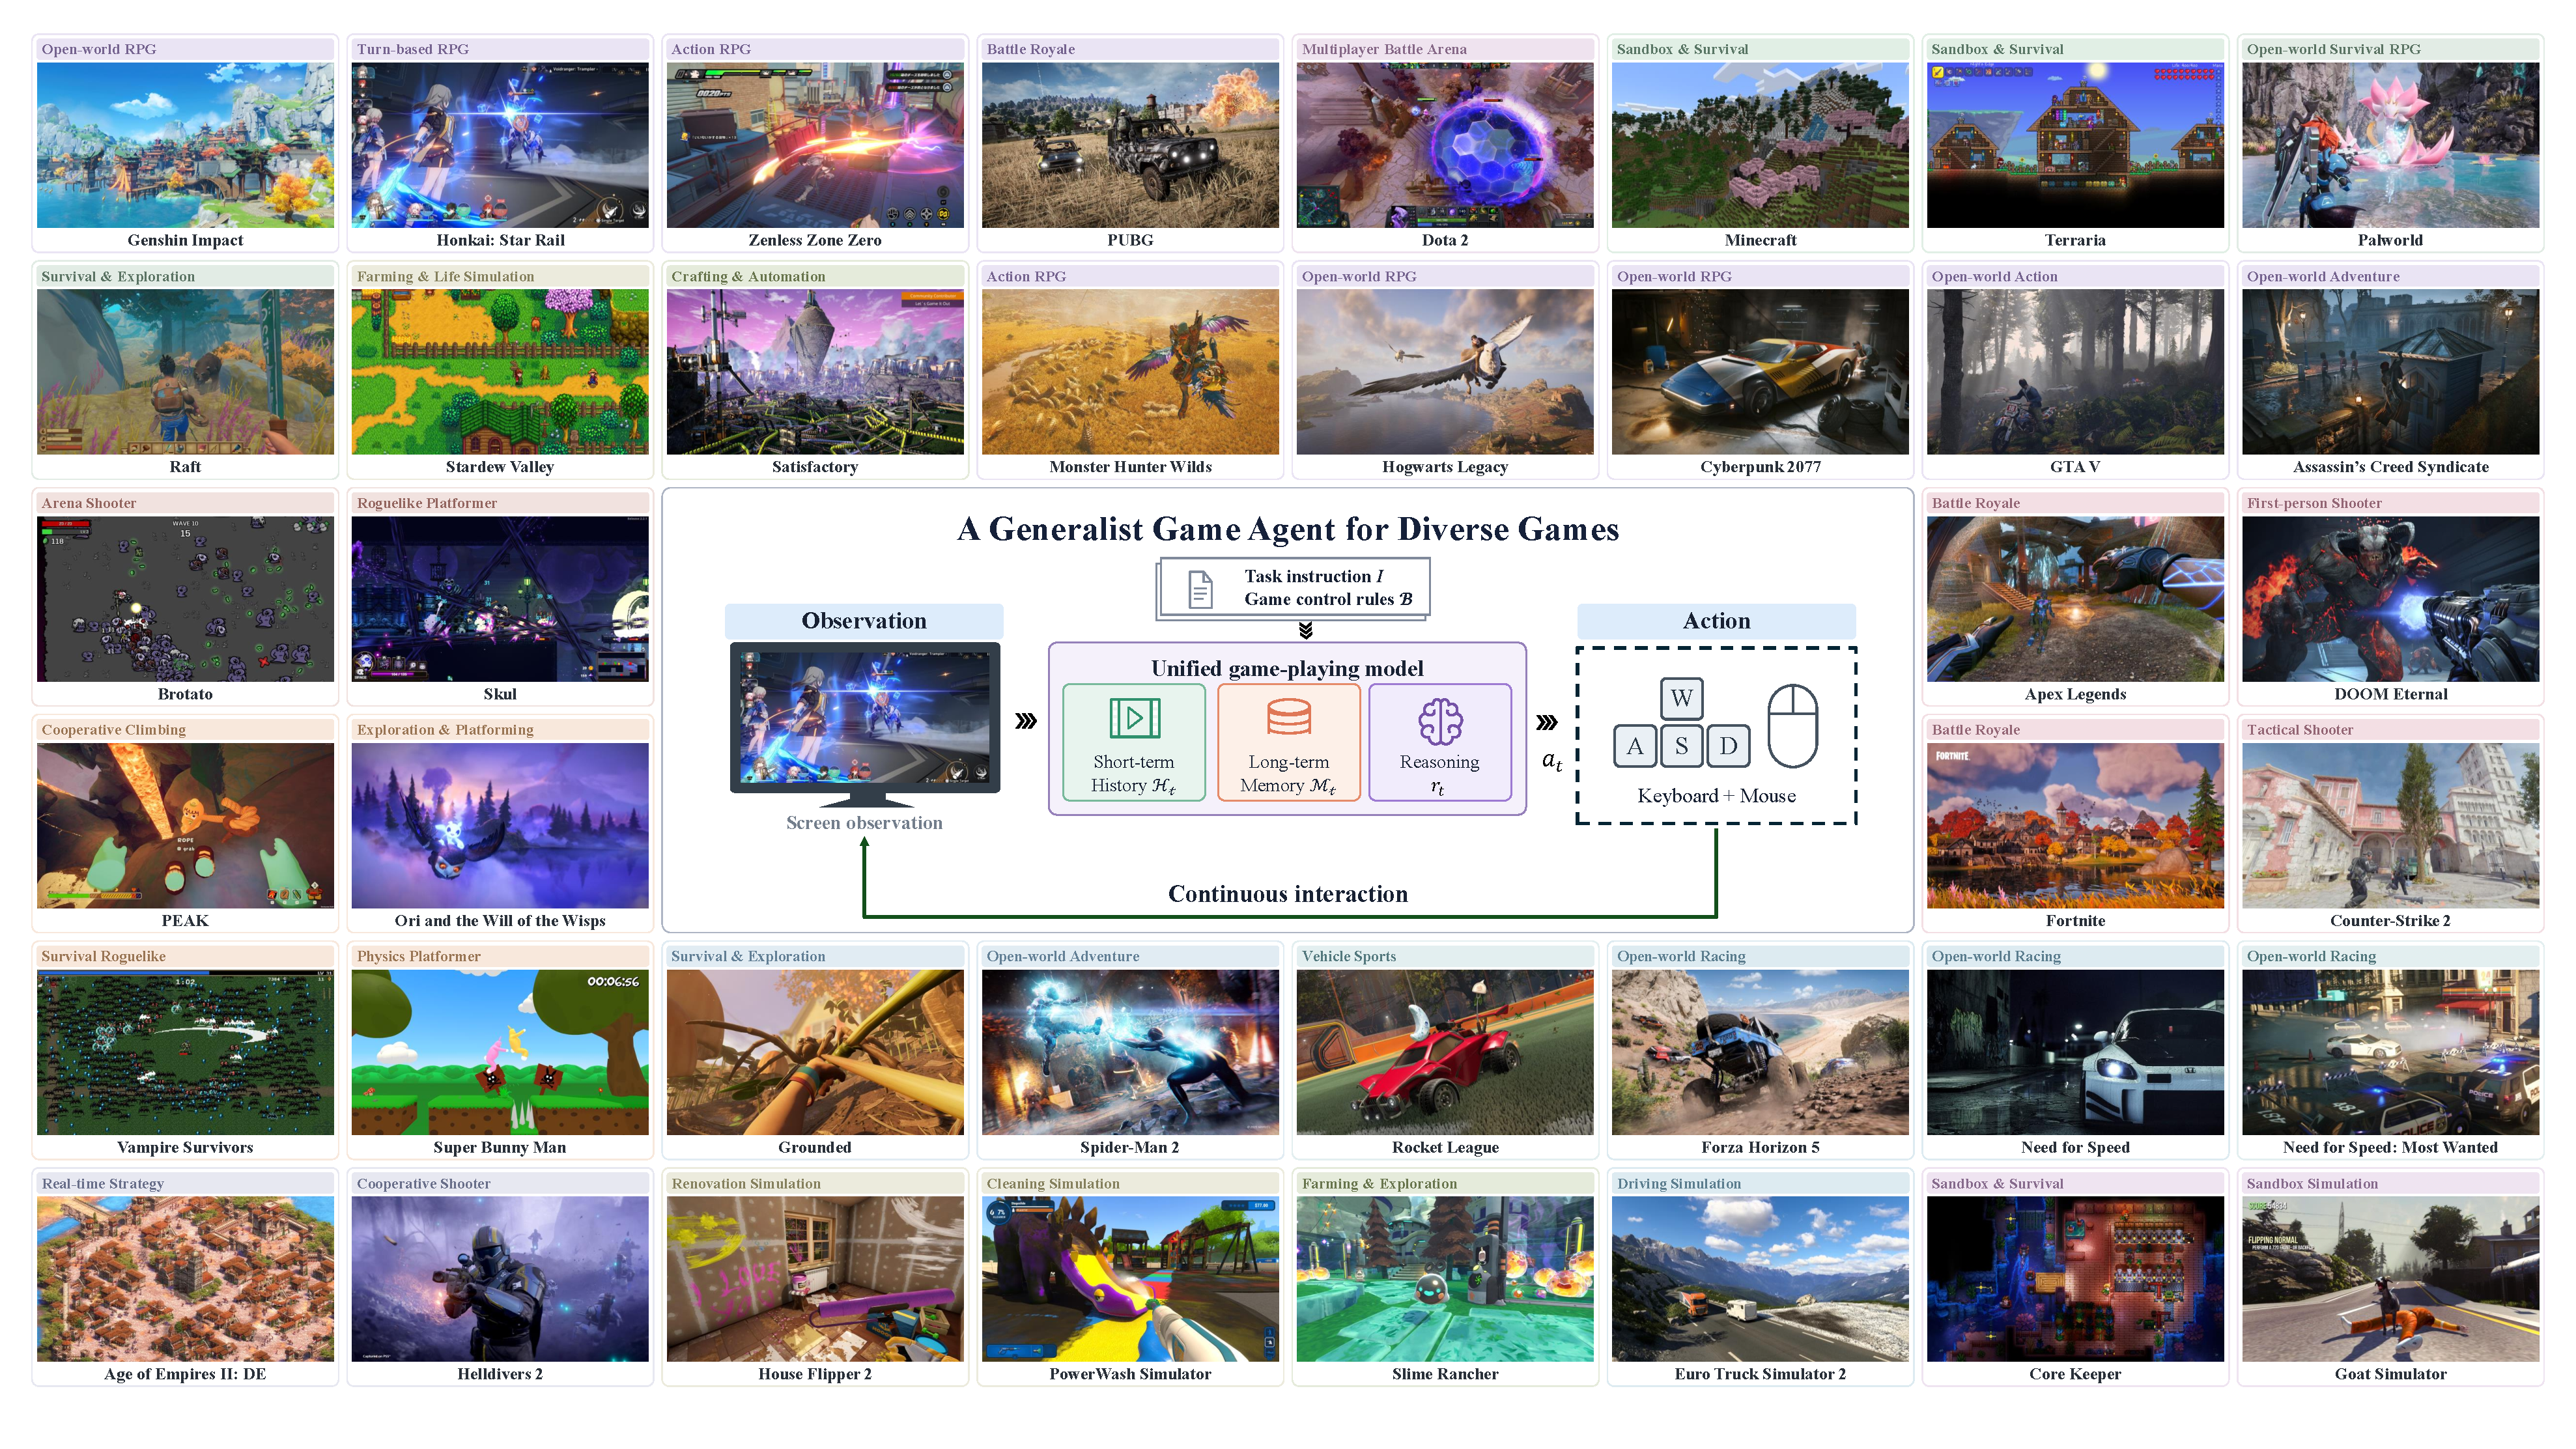
\includegraphics[width=0.91\textwidth]{figs/overview.pdf}
\caption{
\textbf{Overview of \ourmodel.}
A generalist game agent framework operates across a broad range of visually and mechanically diverse games. At each step, the agent uses the current screen, task context, recent interaction history, long-term memory, and reasoning to generate native keyboard and mouse actions in real time. The agent interacts continuously through this loop. Cross-game training, multi-level supervision, and persistent memory support transferable control and sustained task execution.
}
\vspace{-10pt}
\label{fig:overview}
\end{figure*}

\begin{table*}[t]
\centering
\caption{Comparison between \ourmodel and other representative game agents in terms of model initialization, training recipe, training data, real-time inference, and open-source availability. Here, BC, SFT, CPT, and RL denote behavior cloning, supervised fine-tuning, continued pre-training, and reinforcement learning, respectively.}
\label{tab:comparison}
\small
\setlength{\tabcolsep}{8pt}
\renewcommand{\arraystretch}{1.15}
\resizebox{\textwidth}{!}{
\begin{tabular}{@{}lllccc@{}}
\toprule
Method & Initialization & Training Recipe & Training Data & Real-Time & Open-Source \\
\midrule
VPT       & From scratch & BC + RL         & Minecraft      & \ding{51} & \ding{51} \\
Open-P2P  & From scratch & BC              & Diverse        & \ding{51} & \ding{51} \\
NitroGen  & From scratch & BC              & Diverse        & \ding{55} & \ding{51} \\
Game-TARS & Seed-VL-1.5  & CPT + SFT       & Diverse        & \ding{55} & \ding{55} \\
Lumine    & Qwen2-VL     & CPT + SFT       & Genshin Impact & \ding{51} & \ding{55} \\
SIMA 2    & Gemini 2.5 Pro + Flash-Lite & SFT + RL & Diverse & \ding{55} & \ding{55} \\
\midrule
\textbf{\ourmodel (Ours)} & Qwen3.5/Qwen3-VL & CPT + SFT + RL & Diverse & \ding{51} & \ding{51}\textsuperscript{*} \\
\bottomrule
\end{tabular}
}
\vspace{4pt}
\begin{minipage}{\textwidth}
\footnotesize
\raggedright
\textsuperscript{*}For \ourmodel, we release our inference engine
and the checkpoints used in the CPT scaling study.
For data security reasons, we do not release Honkai: Star Rail
data or any model checkpoints trained or fine-tuned on such data.
\end{minipage}
\end{table*}

Although games have long served as standard testbeds for AI, extending these successes to modern, complex games remains challenging. With domain-specific policy optimization, prior agents have matched or exceeded human performance in benchmarks such as Atari~\cite{atari}, Minecraft~\cite{fan2022minedojo}, and StarCraft~\cite{starcraft}. However, these methods typically use privileged internal states, tailored action spaces, or dedicated APIs, which generalize poorly beyond their narrow training domains. As summarized in Table~\ref{tab:comparison}, existing game agents differ substantially in their training recipes, game coverage, and real-time execution capabilities. Because modern games rarely expose internal states or dedicated interaction APIs, a true generalist agent should operate like a human player~\cite{tan2025lumine,wang2025gametars, player1}: perceiving the world through raw visual pixels and acting through standard keyboard-and-mouse interfaces. Unifying transferable control, long-horizon decision-making, and non-invasive execution within a single generalist model remains largely unaddressed.

Unlike static benchmarks, dynamic game environments evolve continuously while an agent observes, reasons, and acts. Therefore, real-time interaction introduces a critical system bottleneck. Conventional inference engines introduce high inference latency, causing actions to be executed after the observed game state has changed. Over long trajectories, these delays can lead to control errors, unnecessary interactions, and early failures. This latency penalty also affects online reinforcement learning (RL): delayed rollouts not only inflate wall-clock collection times but also dilute the quality of policy feedback. Consequently, real-time inference is not merely a deployment requirement, but an important part of effective online learning.

To address these challenges, we present \ourmodel, a scalable generalist agent framework for complex interactive games. \ourmodel observes raw screen pixels and executes native keyboard and mouse controls. This unified device-level interface enables non-invasive interaction across diverse environments, eliminating reliance on game-specific APIs or customized action spaces. We first conduct continued pre-training (CPT) on thousands of hours of multi-source gameplay trajectories and map heterogeneous control formats into a unified keyboard-and-mouse representation to establish a transferable control prior. A scalable data-construction pipeline is built to transform raw gameplay trajectories into multi-level instruction data. Using LLM-assisted annotation, the pipeline adds task instructions, reasoning at critical decisions, and memory summaries while preserving the original observation-action sequences. We produce over a thousand hours of instruction data covering local operations, intermediate subgoals, and complete tasks. We leverage this corpus for sparse-thinking instruction tuning, enabling the policy to organize executable behavior around long-horizon objectives while retaining task-relevant memory. Finally, we introduce Temporal-Aware Group Relative Policy Optimization (TA-GRPO) to further optimize the game policy through online environment feedback and address accumulated execution errors and sparse rewards over extended interactions.

We support large-scale training and real-time deployment through a unified training, evaluation, and inference infrastructure. We extend Verl~\cite{sheng2024hybridflow} to support CPT, SFT, and online RL within a shared training framework, with self-developed Streaming-vLLM serving as the inference engine for interactive evaluation and rollout generation. Streaming-vLLM combines stateful KV-cache reuse, architecture-aware execution, FSM-guided speculative decoding with BF16 verification, and streaming action dispatch to reduce inference latency. Equipped with a sandbox supporting concurrent game instances and a data pipeline that collects trajectories and identifies failures, this system enables iterative policy improvement under real-time interaction constraints. \ourmodel demonstrates solid generalization and operational efficiency comparable to skilled human players on several challenging 3D game tasks and achieves competitive performance on a range of traditional 2D game benchmarks in real-time. These results demonstrate that a unified keyboard-and-mouse action space which is coupled with cross-domain trajectory scaling and real-time online learning can offer a viable pathway toward generalist interactive agents.

We make the following contributions:
\begin{itemize}
    \item \textbf{A generalist agent framework for complex games.}
    \ourmodel interacts with complex game environments non-invasively, using screen images as input and standard keyboard and mouse operations as a unified action space. We demonstrate how learning in this shared action space generalizes across diverse game.

    \item \textbf{A scalable pipeline for long-horizon instruction data construction.}
    We develop a pipeline that transforms multi-source and multi-format gameplay trajectories into instruction data. Through LLM-assisted annotation and quality validation, the pipeline enriches recorded interactions with task instructions, reasoning at critical decisions, and persistent memory summaries. Applied to tens of thousands of hours of gameplay data, it produces over a thousand hours of high-quality instruction data spanning operations, subgoals, and complete quests, providing supervision for long-horizon reasoning and control.

    \item \textbf{Stable and scalable training, evaluation, and real-time inference.}
    We extend Verl into a unified training and evaluation framework spanning CPT, SFT, and TA-GRPO and introduce Streaming-vLLM to support efficient online rollouts and deployment. Our RL approach optimizes memory-linked trajectory segments using verifiable environment feedback at scale.

    \item \textbf{Strong empirical results.}
    \ourmodel demonstrates solid generalization and operational efficiency comparable to skilled human players on challenging 3D commercial game tasks, and achieves competitive performance on several traditional 2D game benchmarks. These results support its potential for industrial-scale deployment.
\end{itemize}